% 2001 年全国新课程卷文科第 19 题：两个元件系统
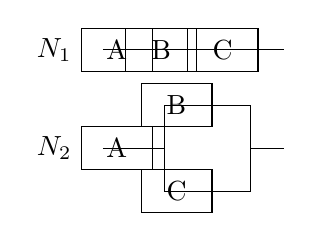
\begin{tikzpicture}[>=stealth, scale=0.78]
  \tikzset{component/.style={draw, rectangle, minimum width=0.9cm,
    minimum height=0.55cm, inner sep=1pt}}
  \node[left] at (0,1.45) {$N_1$};
  \draw (0.35,1.45)--(0.8,1.45)
    node[component, midway] {A}
    --(1.8,1.45)
    node[component, midway] {B}
    --(2.8,1.45)
    node[component, midway] {C}
    --(3.3,1.45);

  \node[left] at (0,-0.15) {$N_2$};
  \draw (0.35,-0.15)--(0.8,-0.15)
    node[component, midway] {A}
    --(1.35,-0.15);
  \draw (1.35,-0.15)--(1.35,0.55)--(1.75,0.55)
    node[component, midway] {B}
    --(2.75,0.55)--(2.75,-0.15);
  \draw (1.35,-0.15)--(1.35,-0.85)--(1.75,-0.85)
    node[component, midway] {C}
    --(2.75,-0.85)--(2.75,-0.15);
  \draw (2.75,-0.15)--(3.3,-0.15);
\end{tikzpicture}
